All code for this section can be found within the appendices.

\subsection{Part 1}

\begin{gather*}
	y[n]=2x[n]-3x[n-1]+2x[n-2] \\
y[n] \text{ in the range } 0 \le n \le 10 \text{ for:} \\
	x[n]=\begin{cases}
		\quad 0   & n < 0 \\
		\quad n+1 & n=0,1,2 \\
		\quad 5-n & n=3,4 \\
		\quad 1   & n\ge 5
	\end{cases}
\end{gather*}

\begin{figure}[H]
	\centering
	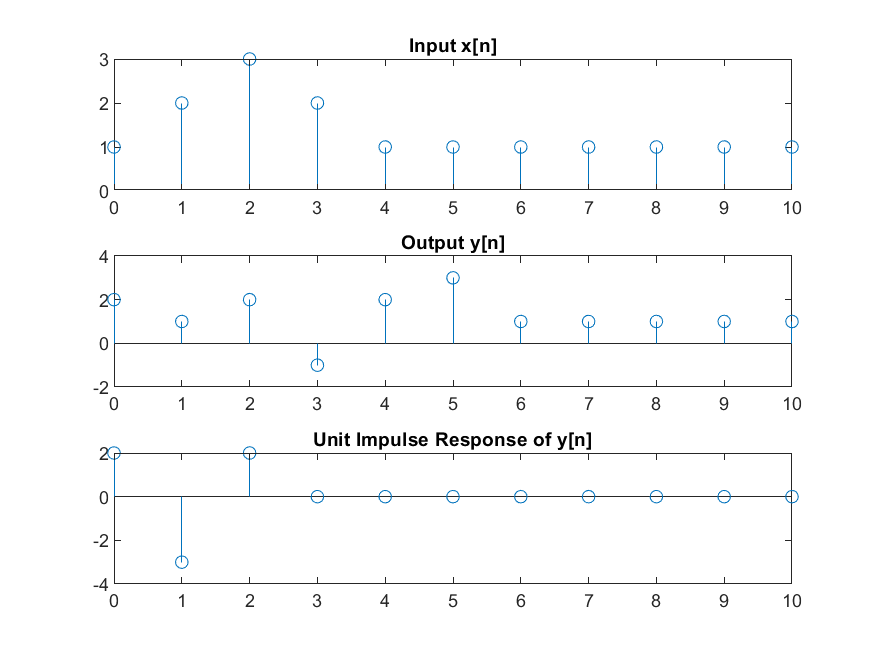
\includegraphics[width=0.8\textwidth]{images/Q1.png}
	\caption{Output for Question 1 Parts 1, 2, and 3}
	\label{fig:Q1Img}
\end{figure}

From Figure \ref{fig:Q1Img} it can be seen that the values for $y[n]$ are
$\{2,1,2,-1,2,3,1,1,1,1,1\}.$

